\subsection{Auswertung des Versuchs Elektronen im elektrischen Feld}
	
	Im Folgenden sind die während der Versuche aufgenommenen Daten
	und die aus diesen berechneten Ergebnisse tabellarisch und graphisch
	dargestellt. An entsprechender Stelle sind Erklärungen zu den 
	durchgeführten Rechnungen und Ergebnissen gegeben.
	Die für die Fehlerrechnung verwendeten Fehlergleichungen befinden 
	sich in \cref{sec:Fehlerrechnung} und sind mit römischen Ziffern nummeriert.

	\subsubsection{Ablenkung von Elektronen in Abhängigkeit der Spannung}
	
		Die während den fünf Messdurchgängen aufgenommenen Werte für die
		Ablenk- und Beschleunigungsspannung sowie die Verschiebung sind in \cref{tab:Auswertung_Messdaten_I} zu finden.
				
			\begin{table}[!h]
	\centering
	\begin{tabular}{|c|c|c|c|}
		\hline
		Pos. Bild & Pos. Linse & Gegenstandsweite & Bildweite\\
		$x_{B}$ [\si{\centi\meter}] & $x_{L}$ [\si{\centi\meter}] & $g$ [\si{\centi\meter}] & $b$ [\si{\centi\meter}]\\
\hline\hline
		\num{89.6(1)} & \num{109.0(1)} & \num{20.0(1)} & \num{19.4(1)}\\
		\num{87.8(1)} & \num{104.0(1)} & \num{25.0(1)} & \num{16.2(1)}\\
		\num{84.4(1)} & \num{99.0(1)} & \num{30.0(1)} & \num{14.6(1)}\\
		\num{80.4(1)} & \num{94.0(1)} & \num{35.0(1)} & \num{13.6(1)}\\
		\num{76.0(1)} & \num{89.0(1)} & \num{40.0(1)} & \num{13.0(1)}\\
		\num{71.5(1)} & \num{84.0(1)} & \num{45.0(1)} & \num{12.5(1)}\\
		\num{66.9(1)} & \num{79.0(1)} & \num{50.0(1)} & \num{12.1(1)}\\
		\num{62.1(1)} & \num{74.0(1)} & \num{55.0(1)} & \num{11.9(1)}\\
		\num{57.2(1)} & \num{69.0(1)} & \num{60.0(1)} & \num{11.8(1)}\\
		\num{52.4(1)} & \num{64.0(1)} & \num{65.0(1)} & \num{11.6(1)}\\
		\hline
	\end{tabular}
	\caption{Gemessene Positionen des Bildes und der Linse und die daraus bestimmten 
		Bild- und Gegenstandsweiten für die Messreihe mit der bekannten Linse. Als Fehler wurde die kleinste Skaleneinteilung des
		verwendeten Millimetermaßes angenommen.  \label{tab:Auswertung_Messwerte_I}}
\end{table}
   
		
		In den folgenden \crefrange{fig:Auswertung_Messdaten_I_I}{fig:Auswertung_Messdaten_I_V} sind die 
		gemessenen Verschiebungen $D$ gegen die entsprechenden Ablenkspannungen $U_{d}$ aufgetragen.
		Die mittels lineare Ausgleichsrechnung mit dem Ansatz 
		\begin{empheq}{equation}
			D(U_{d}) = m \cdot U_{d} + b,
		\end{empheq} 
		unter Verwendung der Python Bibliothek \emph{SciPy} \cite{SciPy},
		berechneten Parameter $m_{i}, b_{i}$ sind in \cref{tab:Auswertung_Parameter_E} aufgelistet.
		
		\begin{table}[!h]
	\centering
	\begin{tabular}{|c|c|}
		\hline
		Steigung & y-Achsenabschnitt\\
		$m$ [\si{\meter\per\volt}] & $b$ [\si{\cm\meter}]\\
\hline\hline
		\num{0.173(2)} & \num{3.69(3)}\\
		\num{0.1082(8)} & \num{3.65(1)}\\
		\num{0.0930(9)} & \num{3.29(2)}\\
		\num{0.084(1)} & \num{3.72(2)}\\
		\num{0.066(1)} & \num{3.67(2)}\\
		\hline
	\end{tabular}
	\caption{Fit-Parameter der Daten aus den fünf Messreihen \label{tab:Auswertung_Parameter_E}}
\end{table}

		
		
		\begin{figure}[!h]
				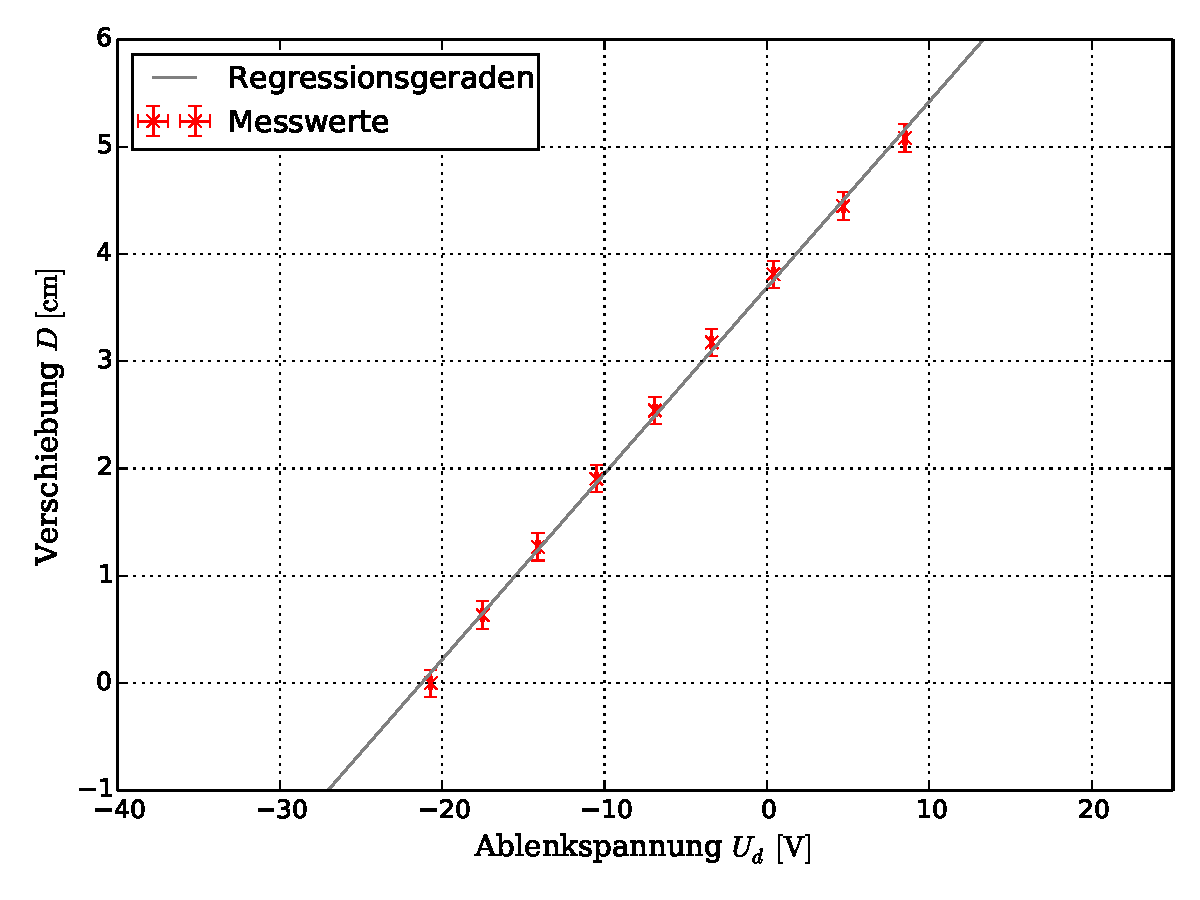
\includegraphics[scale=0.7]{Grafiken/EFeld_Messreihe_I.pdf}
				\caption{Grafische Darstellung der ersten Messreihe}\label{fig:Auswertung_Messdaten_I_I}
		\end{figure}
		
		\begin{figure}[!h]
				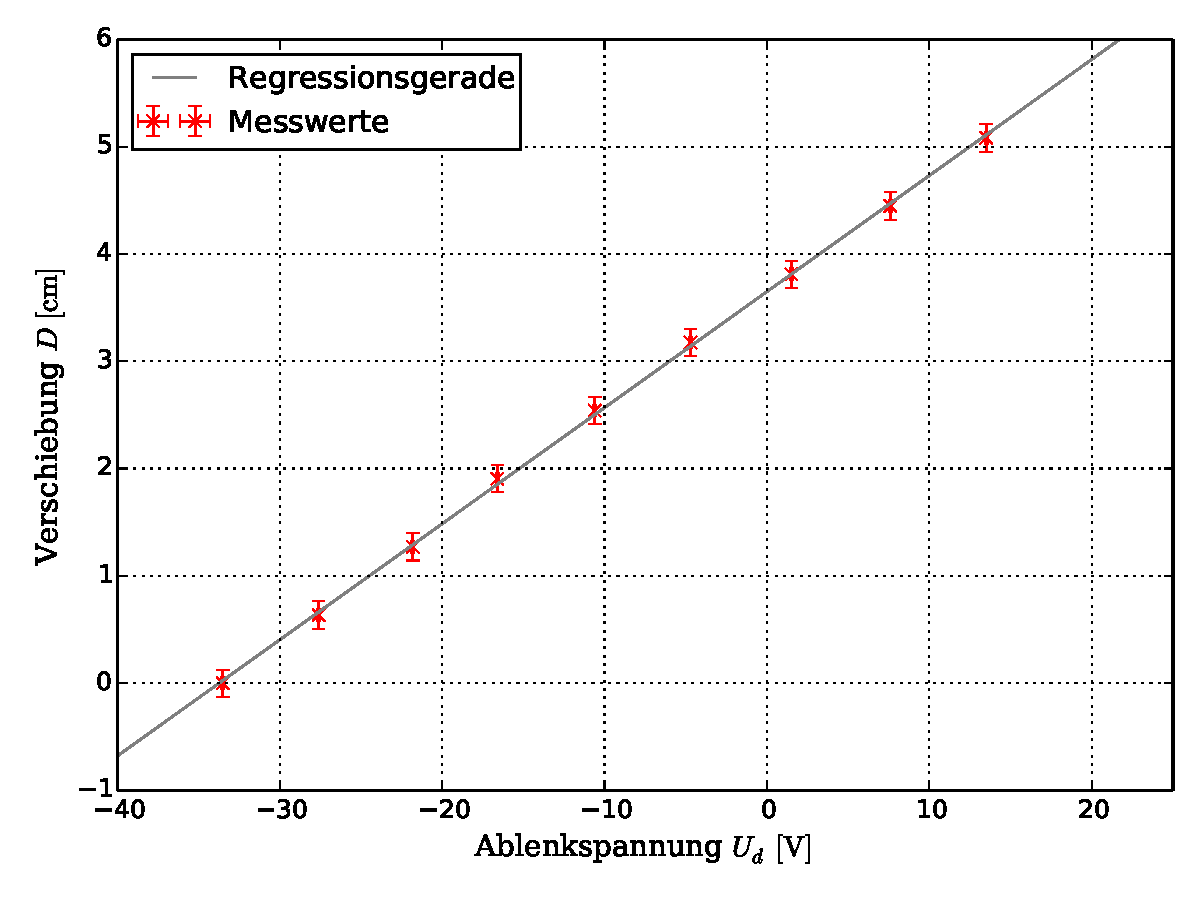
\includegraphics[scale=0.7]{Grafiken/EFeld_Messreihe_II.pdf}
				\caption{Grafische Darstellung der zweiten Messreihe}\label{fig:Auswertung_Messdaten_I_II}
		\end{figure}
		
		\begin{figure}[!h]
				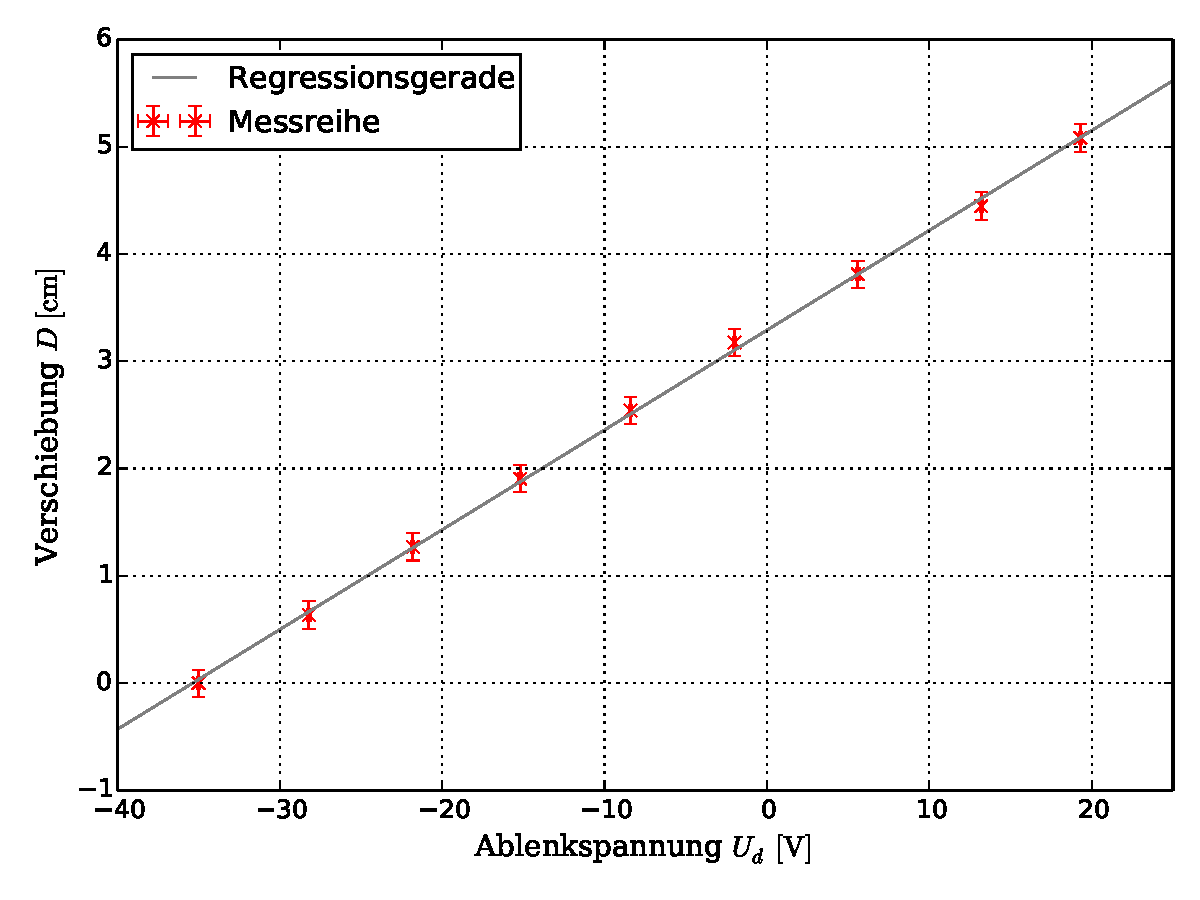
\includegraphics[scale=0.7]{Grafiken/EFeld_Messreihe_III.pdf}
				\caption{Grafische Darstellung der dritten Messreihe}\label{fig:Auswertung_Messdaten_I_III}
		\end{figure}
		
		\begin{figure}[!h]
				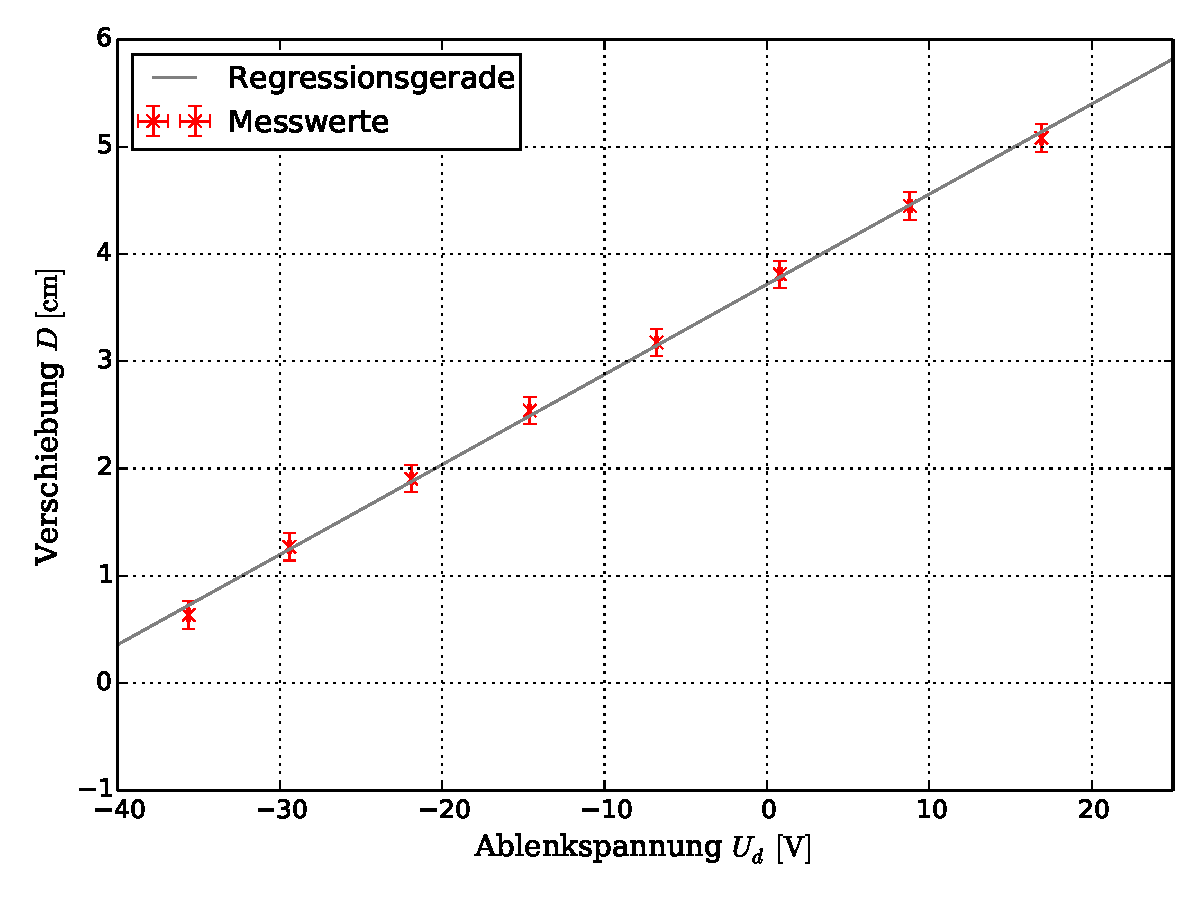
\includegraphics[scale=0.7]{Grafiken/EFeld_Messreihe_IV.pdf}
				\caption{Grafische Darstellung der vierten Messreihe}\label{fig:Auswertung_Messdaten_I_IV}
		\end{figure}
		
		\begin{figure}[!h]
				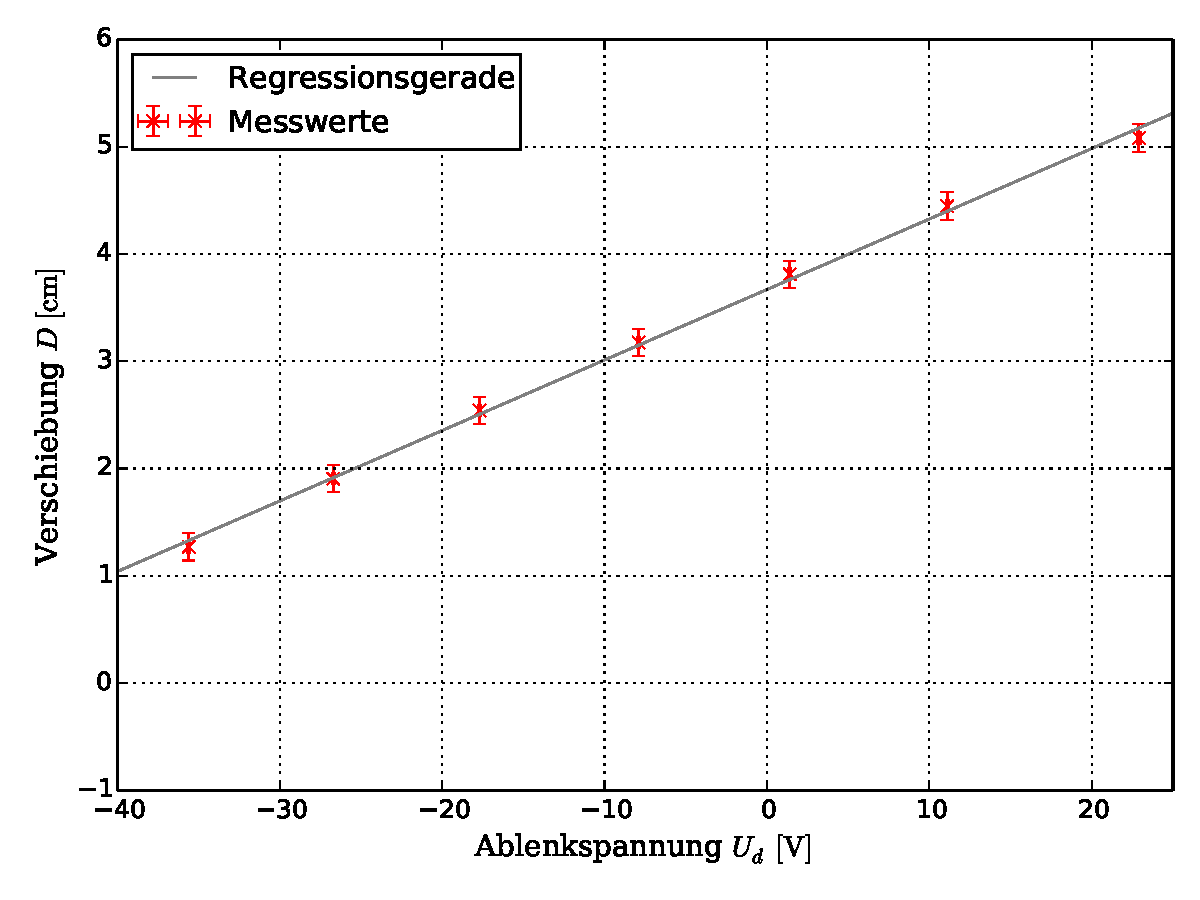
\includegraphics[scale=0.7]{Grafiken/EFeld_Messreihe_V.pdf}
				\caption{Grafische Darstellung der fünften Messreihe}\label{fig:Auswertung_Messdaten_I_V}
		\end{figure}
		
		Die Steigung dieser Graphen stellt die Empfindlichkeit $\frac{D}{U_{d}}$
		der Apparatur dar, die in \cref{fig:Auswertung_} gegen die reziproke 
		Beschleunigungsspannung aus \cref{tab:Auswertung_Messdaten_I} aufgetragen ist.
		
		\begin{figure}[!h]
			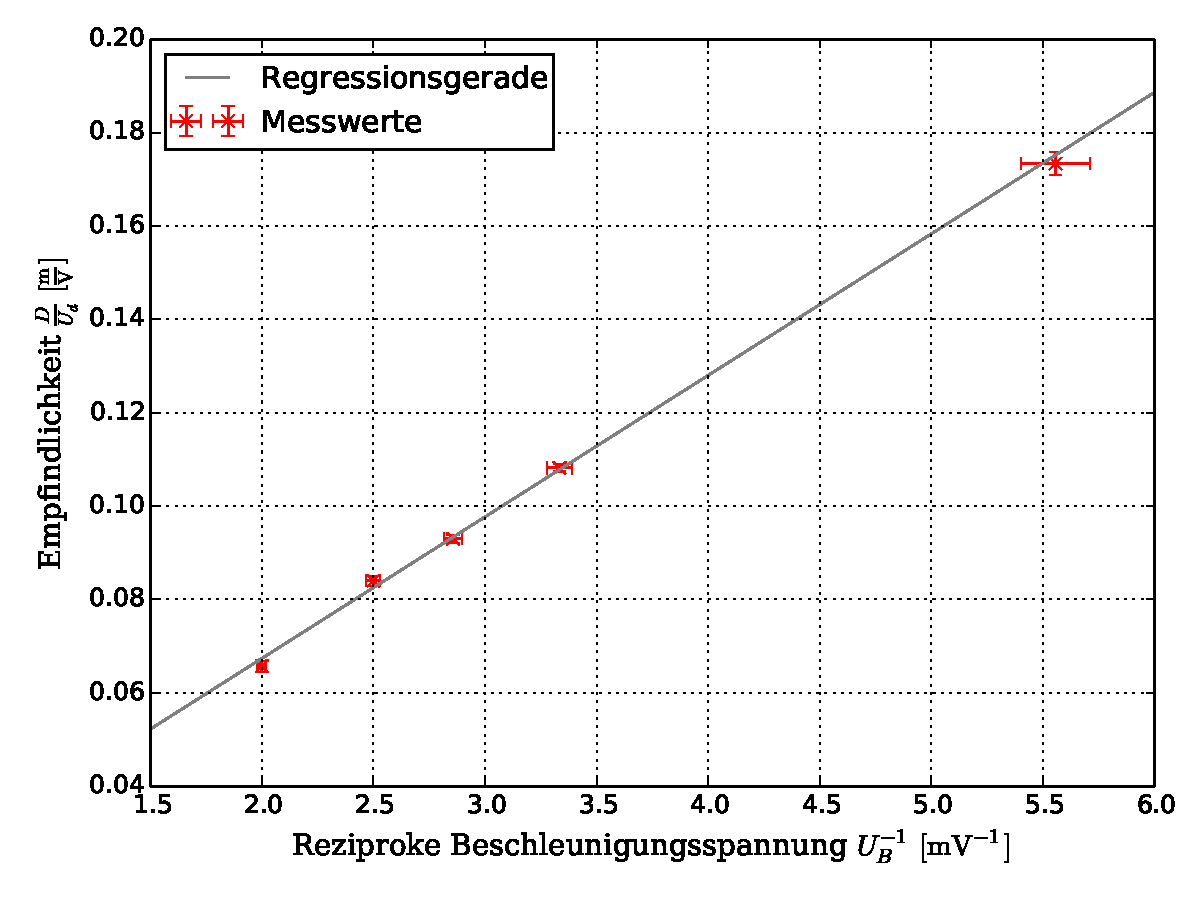
\includegraphics[scale=0.7]{Grafiken/EFeld_Messreihe_VI.pdf}
			\caption{Darstellung des Zusammenhangs von Empfindlichkeit Beschleunigungsspannung}\label{fig:Auswertung_Messdaten_I_VI}
		\end{figure}
		
		Die durch Regression mit dem  Ansatz
		\begin{empheq}{equation}
		e(U_{b}^{-1}) = \frac{c}{U_{b}} + d,
		\end{empheq} 		
		erhält man die Parameter
		\addtocounter{equation}{-1}
		\begin{subequations}
			\begin{empheq}{align} 
				c &= \SI{30.3(8)}{\centi\meter}\\ 
				d &= \SI{0.006(3)}{\centi\meter\per\volt}.
			\end{empheq}
		\end{subequations}
		
		Ein theoretischer Vergleichswert zu dem in \cref{fig:Auswertung_Messdaten_I_VI} 
		dargestellten Zusammenhang erhält man mittels \cref{eq:Theorie_} und den
		Angaben im Bauplan \cite{V501} der Kathodenstrahlröhre zu den Maßen
		$L = \SI{17.5}{\centi\meter}$ und $p = \SI{1.9}{\centi\meter}$.
		Da der Abstand der Platten nicht auf der ganzen Länge des Kondensators
		gleich ist, wird für die angestellte Berechnung der Mittelwert
		\begin{empheq}{equation}
			d = d_{1} \cdot \frac{p_{1}}{p} + 
				\del{\frac{d_{1} + d_{2}}{2}}\cdot \frac{p_{2}}{p} = \SI{0.508}{cm} 
		\end{empheq}
		verwendet. Die für die Berechnung verwendeten Größen sind in 
		\cref{fig:Auswertung_Bauplan} dargestellt. 
		
		Aus den genannten Größen berechnet sich die theoretische Steigung der 
		Geraden in \cref{fig:Auswertung_Messdaten_I_VI} zu
		\begin{empheq}{equation} 
			c_{theo} = \SI{32.71}{\centi\meter}.
		\end{empheq}	
		\begin{figure}[!h]
			\centering
			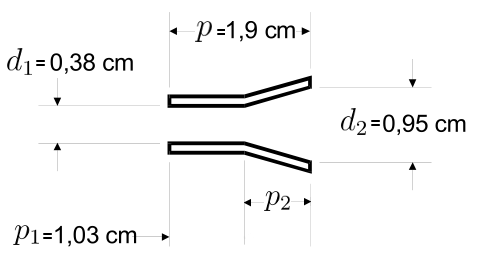
\includegraphics[scale=0.7]{Grafiken/Bauplan.PNG}
			\caption{Bauplan der x-Ablenkung}\label{fig:Auswertung_Bauplan}
		\end{figure}
		
	\subsubsection{Stehende Sinuswellen am rudimentären Oszilloskop}

		

\subsection{Auswertung des Versuchs Elektronen im magnetischen Feld}